% SC3000 --- Chapter 8: Machine Learning (0->100 ground-up)
\chapter{Learning from Data}
\label{ch:learning}

\begin{quote}
\emph{``A program learns from experience $E$ with respect to task $T$ and performance $P$ if its performance on $T$, as measured by $P$, improves with $E$.''} --- Tom Mitchell. We make this concrete: from data to hypotheses, from entropy to trees, from a single neuron to a network.
\end{quote}

\noindent\fbox{\parbox{\dimexpr\linewidth-2\fboxsep-2\fboxrule}{%
\textbf{From zero: no ML assumed.} We build from counting and Ch.~1 agents only: training data as labelled examples, generalisation as the goal, then two pillars---decision trees (discrete, interpretable) and the perceptron (continuous, neural preview). No prior statistics required.}}
\vspace{0.4em}

\section*{Learning Outcomes}
After this chapter you will be able to:
\begin{enumerate}[label=(L\arabic*)]
    \item distinguish supervised, unsupervised, and reinforcement learning;
    \item explain training/test split and overfitting;
    \item compute entropy and information gain and trace ID3;
    \item run $k$-NN and describe the bias of linear hypotheses;
    \item execute the perceptron rule and explain why XOR needs a hidden layer.
\end{enumerate}

% ============================================================
\section{What Is Learning?}
\label{sec:what-is-learning}
An agent with fixed rules fails when the world changes. A \emph{learning} agent improves its mapping $h:\mathcal{X}\to\mathcal{Y}$ from experience. Data are pairs $(x^{(i)},y^{(i)})$ where $x$ is a feature vector and $y$ is the label.

Three regimes differ only in feedback:
\begin{description}[leftmargin=1.2em, itemsep=0.3em]
    \item[Supervised] $(x,y)$ given; learn $h\approx f$. Classification ($y$ discrete) or regression ($y$ continuous).
    \item[Unsupervised] Only $x$ given; find structure (clusters, density).
    \item[Reinforcement] Agent acts, receives reward $r$, must credit actions to rewards.
\end{description}
We focus on supervised learning. Fix a \emph{hypothesis space} $\mathcal{H}$ (e.g., all depth-2 trees). The learner picks $\hat h\in\mathcal{H}$ minimising training error, but we care about \emph{test error} on unseen data. A large $\mathcal{H}$ can memorise training data yet fail on new inputs---\emph{overfitting}. Split data into train/validate/test: fit on train, choose $\mathcal{H}$ on validate, report once on test.

\begin{figure}[h!]
\centering
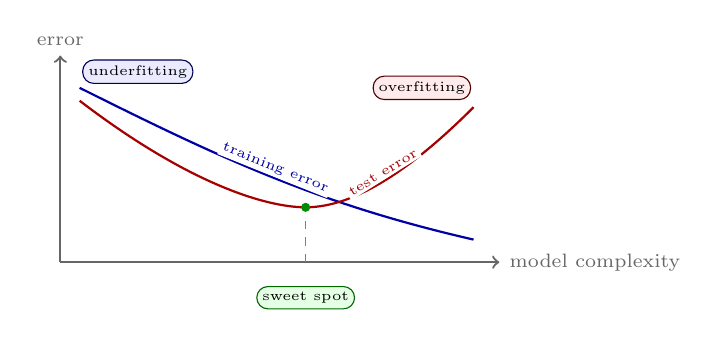
\begin{tikzpicture}[scale=0.82, every node/.style={font=\scriptsize}]
  \draw[->, thick, black!60] (0,0) -- (6.8,0) node[right] {model complexity};
  \draw[->, thick, black!60] (0,0) -- (0,3.2) node[above] {error};
  \draw[thick, blue!65!black] (0.3,2.7) .. controls (2.5,1.6) and (4.0,0.9) .. (6.4,0.35)
    node[midway, above, sloped, font=\tiny, fill=white, inner sep=1pt] {training error};
  \draw[thick, red!65!black] (0.3,2.5) .. controls (2.0,1.2) and (3.2,0.85) .. (3.8,0.85)
    .. controls (4.6,0.85) and (5.5,1.5) .. (6.4,2.4)
    node[midway, above, sloped, font=\tiny, fill=white, inner sep=1pt] {test error};
  \draw[dashed, gray] (3.8,0) -- (3.8,0.85);
  \fill[green!55!black] (3.8,0.85) circle (2pt);
  \node[font=\tiny, fill=green!10, draw=green!40!black, rounded corners, inner sep=2pt] at (3.8,-0.55) {sweet spot};
  \node[font=\tiny, fill=red!8, draw=red!30!black, rounded corners, inner sep=2pt] at (5.6,2.7) {overfitting};
  \node[font=\tiny, fill=blue!8, draw=blue!30!black, rounded corners, inner sep=2pt] at (1.2,2.95) {underfitting};
\end{tikzpicture}
\caption{Training error falls with complexity; test error is U-shaped. The gap is overfitting---memorising noise, not signal.}
\label{fig:overfitting}
\end{figure}

% ============================================================
\section{Decision Trees: Entropy and Information Gain}
\label{sec:decision-trees}
A \emph{decision tree} classifies by asking a sequence of feature tests. Each internal node tests an attribute, each branch is a value, each leaf is a class.

\paragraph{Which attribute first?} The one that reduces uncertainty most. For set $S$ with class proportions $p_c$,
\[
  H(S) = -\sum_c p_c \log_2 p_c \quad\text{(entropy, bits)},
\]
with $0\log 0:=0$. $H=0$ when pure; $H=1$ for a fair coin. Splitting $S$ on attribute $A$ into subsets $S_v$ gives
\[
  \text{Gain}(S,A) = H(S) - \sum_v \frac{|S_v|}{|S|}\,H(S_v).
\]
ID3 greedily picks $\arg\max_A \text{Gain}(S,A)$ and recurses.

\begin{figure}[h!]
\centering
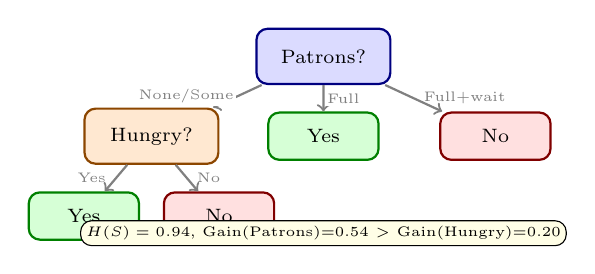
\begin{tikzpicture}[scale=0.78, every node/.style={font=\scriptsize},
  dnode/.style={draw, thick, rounded corners, fill=blue!14, draw=blue!50!black, align=center, minimum width=1.7cm, minimum height=0.7cm},
  leaf/.style={draw, thick, rounded corners, fill=green!16, draw=green!50!black, align=center, minimum width=1.4cm, minimum height=0.6cm},
  edge/.style={->, thick, black!50}]
  \node[dnode] (root) at (4,3.0) {Patrons?};
  \node[dnode, fill=orange!18, draw=orange!55!black] (hungry) at (1.2,1.7) {Hungry?};
  \node[leaf] (yes1) at (4,1.7) {Yes};
  \node[leaf, fill=red!12, draw=red!50!black] (no1) at (6.8,1.7) {No};
  \node[leaf] (yes2) at (0.1,0.4) {Yes};
  \node[leaf, fill=red!12, draw=red!50!black] (no2) at (2.3,0.4) {No};
  \draw[edge] (root) -- (hungry) node[midway, left, font=\tiny, fill=white, inner sep=1pt] {None/Some};
  \draw[edge] (root) -- (yes1) node[midway, right, font=\tiny, fill=white, inner sep=1pt] {Full};
  \draw[edge] (root) -- (no1) node[midway, right, font=\tiny] {Full+wait};
  \draw[edge] (hungry) -- (yes2) node[midway, left, font=\tiny] {Yes};
  \draw[edge] (hungry) -- (no2) node[midway, right, font=\tiny] {No};
  \node[font=\tiny, fill=yellow!10, draw, rounded corners, inner sep=2pt] at (4,0.12) {$H(S)=0.94$, Gain(Patrons)=0.54 $>$ Gain(Hungry)=0.20};
\end{tikzpicture}
\caption{Decision tree for the restaurant domain. Root splits on Patrons because it maximises gain. Green = positive, red = negative.}
\label{fig:dectree}
\end{figure}

\begin{example}[Entropy calculation]
$12$ examples: $6$ Yes, $6$ No gives $H(S)=1$ bit. Splitting on Patrons yields None ($0$Y,$2$N, $H=0$), Some ($4$Y,$0$N, $H=0$), Full ($2$Y,$4$N, $H=0.92$). Weighted entropy $=0.46$, so Gain $=0.54$ bits.
\end{example}

$k$-NN is the opposite extreme: no tree, just vote among the $k$ nearest training points (Euclidean distance). Small $k$ overfits; large $k$ over-smooths. Linear regression fits $\hat y=w^{\top}x+b$ by minimising squared error via gradient descent---the same update shape the perceptron uses.

\begin{lstlisting}[language=Python, caption={ID3 decision-tree learner (categorical features)}, label={lst:id3}]
import math
from collections import Counter

def entropy(labels):
    n = len(labels)
    return -sum((c/n)*math.log2(c/n) for c in Counter(labels).values())

def info_gain(data, attr, label_key='y'):
    base = entropy([r[label_key] for r in data])
    vals = set(r[attr] for r in data)
    weighted = sum(len([r for r in data if r[attr]==v])/len(data)
                   * entropy([r[label_key] for r in data if r[attr]==v])
                   for v in vals)
    return base - weighted

data = [
    {'Patrons':'None','Hungry':'Yes','y':'No'},
    {'Patrons':'Some','Hungry':'Yes','y':'Yes'},
    {'Patrons':'Full','Hungry':'Yes','y':'Yes'},
    {'Patrons':'Full','Hungry':'No','y':'No'},
]
print("Gain(Patrons)=%.2f" % info_gain(data, 'Patrons'))
print("Gain(Hungry)=%.2f" % info_gain(data, 'Hungry'))
\end{lstlisting}

% ============================================================
\section{The Perceptron and Neural Preview}
\label{sec:perceptron}
A \emph{perceptron} is one artificial neuron. With inputs $x$, weights $w$, bias $b$,
\[
  z = w\cdot x + b,\qquad \hat y = \begin{cases}1 & z\ge 0\\ 0 & z<0\end{cases}
\]
so $\hat y=\text{step}(z)$. Geometrically, $w\cdot x+b=0$ is a hyperplane separating classes.

\paragraph{Learning rule.} On mistake $(x,y)$, $y\in\{0,1\}$,
\[
  w \leftarrow w + \eta\,(y-\hat y)\,x,\qquad b \leftarrow b + \eta\,(y-\hat y),
\]
with rate $\eta>0$. If data are linearly separable, this converges in finite steps (Block--Novikoff). Otherwise it cycles---XOR is the classic impossibility: no single line separates $\{(0,0),(1,1)\}$ from $\{(0,1),(1,0)\}$.

\begin{figure}[h!]
\centering
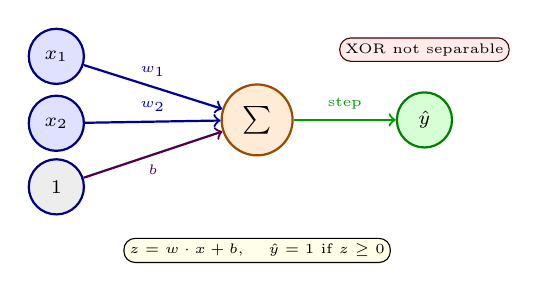
\begin{tikzpicture}[scale=0.85, every node/.style={font=\scriptsize},
  inp/.style={circle, draw, thick, minimum size=0.7cm, fill=blue!12, draw=blue!50!black},
  sumnode/.style={circle, draw, thick, minimum size=0.9cm, fill=orange!16, draw=orange!60!black},
  outnode/.style={circle, draw, thick, minimum size=0.7cm, fill=green!16, draw=green!50!black}]
  \node[inp] (x1) at (0,1.4) {$x_1$};
  \node[inp] (x2) at (0,0.4) {$x_2$};
  \node[inp, fill=gray!14] (b) at (0,-0.55) {$1$};
  \node[sumnode] (s) at (3.0,0.45) {$\sum$};
  \node[outnode] (y) at (5.5,0.45) {$\hat y$};
  \draw[->, thick, blue!60!black] (x1) -- (s) node[midway, above, font=\tiny] {$w_1$};
  \draw[->, thick, blue!60!black] (x2) -- (s) node[midway, above, font=\tiny] {$w_2$};
  \draw[->, thick, violet!60!black] (b) -- (s) node[midway, below, font=\tiny] {$b$};
  \draw[->, thick, green!60!black] (s) -- (y) node[midway, above, font=\tiny] {step};
  \node[font=\tiny, fill=yellow!10, draw, rounded corners, inner sep=2pt] at (3.0,-1.5) {$z=w\cdot x+b$, \quad $\hat y=1$ if $z\ge 0$};
  \node[font=\tiny, fill=red!8, draw=red!30!black, rounded corners, inner sep=2pt] at (5.5,1.5) {XOR not separable};
\end{tikzpicture}
\caption{Perceptron as a linear separator. Stacking such units with non-linear activations gives a multi-layer network that solves XOR.}
\label{fig:perceptron}
\end{figure}

Stacking perceptrons with a smooth activation (sigmoid, ReLU) yields a \emph{feed-forward network}. With one hidden layer it is a universal approximator; training via gradient descent (backpropagation) minimises cross-entropy---the bridge to deep learning.

\begin{lstlisting}[language=Python, caption={Perceptron learning rule from scratch}, label={lst:perceptron}]
import numpy as np

def perceptron_train(X, y, eta=0.1, epochs=20):
    """X: (n,d) array, y in {0,1}. Returns (w,b)."""
    n, d = X.shape
    w = np.zeros(d)
    b = 0.0
    for _ in range(epochs):
        err = 0
        for xi, yi in zip(X, y):
            yhat = 1 if np.dot(w, xi) + b >= 0 else 0
            if yhat != yi:
                w += eta * (yi - yhat) * xi
                b += eta * (yi - yhat)
                err += 1
        if err == 0:
            break  # converged: linearly separable
    return w, b

X_and = np.array([[0,0],[0,1],[1,0],[1,1]])
y_and = np.array([0,0,0,1])
y_xor = np.array([0,1,1,0])
print("AND w:", perceptron_train(X_and, y_and)[0])
w, b = perceptron_train(X_and, y_xor, epochs=10)
print("XOR solved?", np.all(((X_and.dot(w)+b)>=0).astype(int)==y_xor))
\end{lstlisting}

\section{Sequential Decisions: MDPs and Reinforcement Learning}
Some tasks give no labels, only rewards: a game agent wins or loses long after acting.
A \emph{Markov decision process} has states $s$, actions $a$, transitions $P(s' \mid s,a)$,
rewards $R(s,a)$, and discount $\gamma \in [0,1)$. A policy $\pi(a \mid s)$ picks actions;
its value $V^{\pi}(s)$ is the expected discounted return from $s$. Bellman intuition: the
value of $s$ is the immediate reward plus the discounted value of wherever we land,
\begin{equation}
V^{\star}(s) = \max_a \sum_{s'} P(s' \mid s, a)\,[R(s,a) + \gamma V^{\star}(s')].
\end{equation}
\emph{Q-learning} learns $Q(s,a)$ without knowing $P$: after observing $(s,a,r,s')$,
\begin{equation}
Q(s,a) \gets Q(s,a) + \alpha\,[r + \gamma \max_{a'} Q(s',a') - Q(s,a)].
\end{equation}
Worked step: $Q(s,\text{up})=1.0$, reward $r=0$, $\gamma=0.9$, $\alpha=0.5$, best next
$\max_{a'}Q(s',a')=2.0$: target $0+0.9 \times 2.0=1.8$, so $Q \gets 1.0+0.5(1.8-1.0)=1.4$.
\begin{lstlisting}[language=Python, caption={Tabular Q-learning update}, label={lst:qlearn}]
def q_update(Q, s, a, r, s_next, alpha=0.5, gamma=0.9):
    """One Q-learning step. Q[(s,a)] -> float; s_next actions from legal(s_next)."""
    best_next = max((Q.get((s_next, ap), 0.0) for ap in legal(s_next)), default=0.0)
    Q[(s, a)] = Q.get((s, a), 0.0) + alpha * (r + gamma * best_next - Q.get((s, a), 0.0))
# grid step above: q_update(Q, s, 'up', 0.0, s_next) moves Q[(s,'up')] 1.0 -> 1.4
\end{lstlisting}
% ============================================================
\section{Key Takeaways}
Supervised learning picks $\hat h\in\mathcal{H}$ to minimise training error but is judged on test error; overfitting grows with $\mathcal{H}$ complexity. Decision trees greedily maximise information gain and are interpretable but need pruning. The perceptron learns a linear separator by mistake-driven updates and converges iff data are separable; stacking units with non-linearities yields deep networks trained by gradient descent.

% ============================================================
\section{Chapter Notes}
Further reading: Russell \& Norvig Ch.~18--19; Mitchell Ch.~3 (trees) and Ch.~4 (perceptron); Goodfellow et al.\ Ch.~6 for deep nets. Try scikit-learn for trees/$k$-NN and PyTorch for perceptrons/MLPs; always report validation curves, not just training accuracy.

% ============================================================
\section{Exercises}
\label{sec:ch08-ex}
\begin{enumerate}[label=E8.\arabic*, leftmargin=*, itemsep=0.7em]
    \item \textbf{Paradigms.} For (a) spam filter from labelled emails, (b) customer segmentation from purchase histories, (c) game agent from win/loss rewards, state the regime (supervised/unsupervised/RL) and what $(x,y)$ or reward is.
    \item \textbf{Entropy and gain.} Dataset $S$: 9 Yes, 5 No. Attribute $A$ splits into $\{6Y,1N\}$ and $\{3Y,4N\}$. Compute $H(S)$, $H(S_v)$, and Gain$(S,A)$ in bits. Should $A$ be chosen over $B$ with Gain $0.05$?
    \item \textbf{Overfitting.} A depth-10 tree gets 99\% train and 62\% test accuracy. Name the phenomenon and give two remedies. What does Fig.~\ref{fig:overfitting} predict if depth goes to $15$?
    \item \textbf{Perceptron trace.} Run the perceptron ($\eta=1$, $w=[0,0],b=0$) on $(1,1)\!\to\!1$, $(-1,0)\!\to\!0$, $(0.5,0.5)\!\to\!1$ in order. Show each update and final $w,b$.
    \item \textbf{XOR and depth.} Prove no single perceptron separates XOR. Sketch a 2-hidden-unit network that does: give weights for OR and NAND hidden units and an AND output. Why is non-linearity essential?
\end{enumerate}
% End of Chapter 8
